%% ****** Start of file template.aps ****** %
%%
%%
%%   This file is part of the APS files in the REVTeX 4 distribution.
%%   Version 4.0 of REVTeX, August 2001
%%
%%
%%   Copyright (c) 2001 The American Physical Society.
%%
%%   See the REVTeX 4 README file for restrictions and more information.
%%
%
% This is a template for producing manuscripts for use with REVTEX 4.0
% Copy this file to another name and then work on that file.
% That way, you always have this original template file to use.
%
% Group addresses by affiliation; use superscriptaddress for long
% author lists, or if there are many overlapping affiliations.
% For Phys. Rev. appearance, change preprint to twocolumn.
% Choose pra, prb, prc, prd, pre, prl, prstab, or rmp for journal
%  Add 'draft' option to mark overfull boxes with black boxes
%  Add 'showpacs' option to make PACS codes appear
%  Add 'showkeys' option to make keywords appear
\documentclass{revtex4}
%\documentclass[aps,prl,preprint,superscriptaddress]{revtex4}
%\documentclass[aps,prl,twocolumn,groupedaddress]{revtex4}
\usepackage[dvipdf]{graphicx}
%\usepackage{dcolumn}

% You should use BibTeX and apsrev.bst for references
% Choosing a journal automatically selects the correct APS
% BibTeX style file (bst file), so only uncomment the line
% below if necessary.
%\bibliographystyle{apsrev}

\begin{document}

% Use the \preprint command to place your local institutional report
% number in the upper righthand corner of the title page in preprint mode.
% Multiple \preprint commands are allowed.
% Use the 'preprintnumbers' class option to override journal defaults
% to display numbers if necessary
%\preprint{}

%Title of paper
\title{Measurement of the Velocity of Light in Air}

% repeat the \author .. \affiliation  etc. as needed
% \email, \thanks, \homepage, \altaffiliation all apply to the current
% author. Explanatory text should go in the []'s, actual e-mail
% address or url should go in the {}'s for \email and \homepage.
% Please use the appropriate macro foreach each type of information

% \affiliation command applies to all authors since the last
% \affiliation command. The \affiliation command should follow the
% other information
% \affiliation can be followed by \email, \homepage, \thanks as well.
\author{Physics 2501: Mechanics and Electromagnetism Laboratory}
%\homepage[]{Your web page}
%\thanks{}
%\altaffiliation{}
\affiliation{Dept. of Physics, University of Connecticut}
%\author{R.T. Jones}
%\affiliation{University of Connecticut}

%Collaboration name if desired (requires use of superscriptaddress
%option in \documentclass). \noaffiliation is required (may also be
%used with the \author command).
%\collaboration can be followed by \email, \homepage, \thanks as well.
%\collaboration{}
%\noaffiliation

\date{\today}

%\begin{abstract}
% insert abstract here
%\end{abstract}

% insert suggested PACS numbers in braces on next line
%\pacs{}
% insert suggested keywords - APS authors don't need to do this
%\keywords{}

%\setlength{\topmargin}{0in}

%\maketitle must follow title, authors, abstract, \pacs, and \keywords
\maketitle

% body of paper here - Use proper section commands
% References should be done using the \cite, \ref, and \label commands

%% The normal text is displayed in two-column format, but special
%% sections spanning both columns can be inserted within the page
%% format so that long equations can be displayed. Use
%% sparingly.
%%\begin{widetext}
%% put long equation here
%%\end{widetext}
%
%% figures should be put into the text as floats.
%% Use the graphics or graphicx packages (distributed with LaTeX2e)
%% and the \includegraphics macro defined in those packages.
%% See the LaTeX Graphics Companion by Michel Goosens, Sebastian Rahtz,
%% and Frank Mittelbach for instance.
%%
%% Here is an example of the general form of a figure:
%% Fill in the caption in the braces of the \caption{} command. Put the label
%% that you will use with \ref{} command in the braces of the \label{} command.
%% Use the figure* environment if the figure should span across the
%% entire page. There is no need to do explicit centering.
%
%%\begin{turnpage}
%% Surround figure environment with turnpage environment for landscape
%% figure
%% \begin{turnpage}
%% \begin{figure}
%% \includegraphics{}%
%% \caption{\label{}}
%% \end{figure}
%% \end{turnpage}
%
%% tables should appear as floats within the text
%%
%% Here is an example of the general form of a table:
%% Fill in the caption in the braces of the \caption{} command. Put the label
%% that you will use with \ref{} command in the braces of the \label{} command.
%% Insert the column specifiers (l, r, c, d, etc.) in the empty braces of the
%% \begin{tabular}{} command.
%% The ruledtabular enviroment adds doubled rules to table and sets a
%% reasonable default table settings.
%% Use the table* environment to get a full-width table in two-column
%% Add \usepackage{longtable} and the longtable (or longtable*}
%% environment for nicely formatted long tables. Or use the the [H]
%% placement option to break a long table (with less control than 
%% in longtable).
%
%
%% Surround table environment with turnpage environment for landscape
%% table
%% \begin{turnpage}
%% \begin{table}
%% \caption{\label{}}
%% \begin{ruledtabular}
%% \begin{tabular}{}
%% \end{tabular}
%% \end{ruledtabular}
%% \end{table}
%% \end{turnpage}
%
%% Specify following sections are appendices. Use \appendix* if there
%% only one appendix.
%%\appendix
%%\section{}
%

\section{Introduction}

The velocity of light is an important quantity in physics, both because of
its fundamental role in the theory of the electromagnetic force, and because
it serves to define the fundamental unit of length.  Nearly all physics
experiments involve some kind of distance measurement, and all measurements
of length, from the microscopic charge radius of a proton to the astronomical
distance to a remote galaxy, depend for their validity on the principal that
light pulses travel through vacuum at a constant speed which is independent
of the motion of either the observer or the source.  This speed is usually
denoted as $c$.  

The principle that light pulses require a finite time to travel from a source
to a receiver was not always believed by scientists.  Early attempts to 
measure a delay in the propagation of a light pulse between sources and
receivers on the earth indicated delays that are consistent with zero.  One
famous example of such an experiment was carried out by the astronomer Galileo.
He had an associate stand with a lantern on a distant hill, while Galileo
stood with his own lantern on another hilltop within eyesight of the first.
Galileo's associate was instructed to cover his lantern as soon as he saw
the light from Galileo's lantern go out.  Galileo measured the delay between
the instant that he covered his own lantern and when the glimmer from his
associate's lantern disappeared, interpreting this delay as the round-trip
time of a light pulse.  Given the uncertainty introduced by the human reaction
time, Galileo's result was consistent with zero, leading only to a lower 
bound on what the speed of light might be.

The first successful measurement of a finite velocity of light was made by
Danish Astronomer Olaf Roemer in 1675. Roemer based his measurement on the
observations of the eclipses of one of the moons of Jupiter. He noticed that
the duration of these eclipses was shorter when the earth was moving toward
Jupiter than when the Earth was moving away, and correctly interpreted the
results as resulting from the Doppler effect.  Based upon this interpretation
and his knowledge of the radii and speeds of the orbiting planets, he was able
to measure a finite value for the velocity of light. From observations of the
eclipses over many years, he determined that the velocity of light was
$2.1\times 10^8$~m/s.

In 1849, the French scientist Fizeau was the first to successfully measure
the speed of light over terrestrial distances. He used a rapidly revolving
cogwheel to chop a beam of light into short pulses. A distant mirror reflected
this light back to the rotating cogwheel. Depending on the position of the
cogwheel when the light pulse returned, it would either block the pulse
of light or pass it through to an observer. Using this method, Fizeau measured
the velocity of light to be $3.15\times 10^8$~m/s.
Foucault improved upon Fizeau's method by using a rotating mirror instead of
a cogwheel.  In 1878, Michelson modified the geometry of Foucault's method
to measure a remarkably accurate value for the velocity of light. The best
of his measurements~\cite{Bates88} gave a value of $2.99774\times 10^8$~m/s,
which is close to the currently accepted value of $2.99792458\times 10^8$~m/s.
Michelson's method is the one that is used in this experiment.

\section{Experimental Method}

\begin{figure}
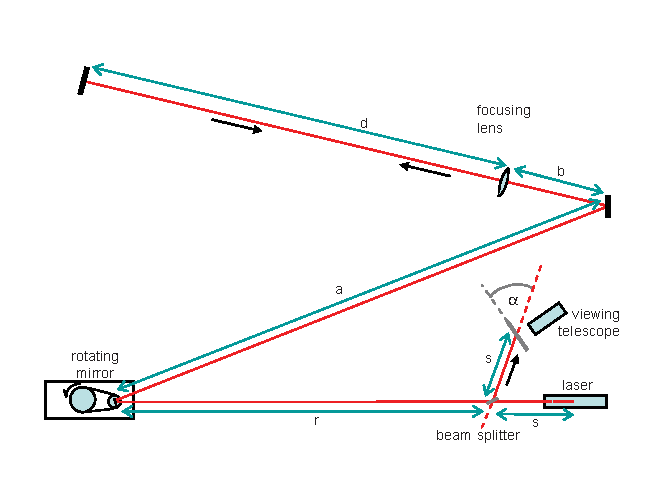
\includegraphics[width=4in]{clightsetup.eps}
\caption{\label{clightsetup}
Diagram of the experimental setup used to measure the speed of light in
air.  The light beam is produced in the laser, passes straight through the
glass slide beam splitter, and reflects from a small mirror mounted on a
rotating spindle.  It then bounces between a couple of mirrors and returns
along its outgoing path back to the laser.  A fraction of the return beam
is reflected from the beam splitter and directed onto a frosted glass
screen.  The spot on the screen is viewed through a telescope that is
equipped with a scale for reading off the position of the spot and 
measuring its displacement as a function of the angular speed of the
rotating mirror.}
\end{figure}

The overall layout of the apparatus is shown in Fig.~\ref{clightsetup}.
Light from the He-Ne laser passes through a partially reflecting beam splitter
and then strikes the rotating mirror.  Bouncing from the mirror, it passes
across the room through a focusing lens onto a second flat mirror.  From the
second mirror it passes back across the room to a final mirror which is
carefully aligned to make the beam retrace its original path back to the
laser.  Before it gets back to the laser, some of the return beam is 
reflected from the beam splitter and directed onto a frosted glass screen.
The light spot on the frosted glass screen is viewed from the back through
a telescope, as shown in the figure.  If the rotating mirror is turning at
a constant velocity then its rotation angle changes by a tiny amount between
the instant that a light pulse is reflected on its outgoing path and when it
is reflected on its return path.  This produces a small shift in the position
of the beam spot on the frosted glass screen which is proportional to the
round-trip time of a light pulse between the two instances that it reflects
from the rotating mirror.  Measuring the round-trip time in this way and
knowing the distances $r$, $s$, $a$, $b$, and $d$ in the figure, a value for
the speed of light in air can be determined.

\begin{figure}
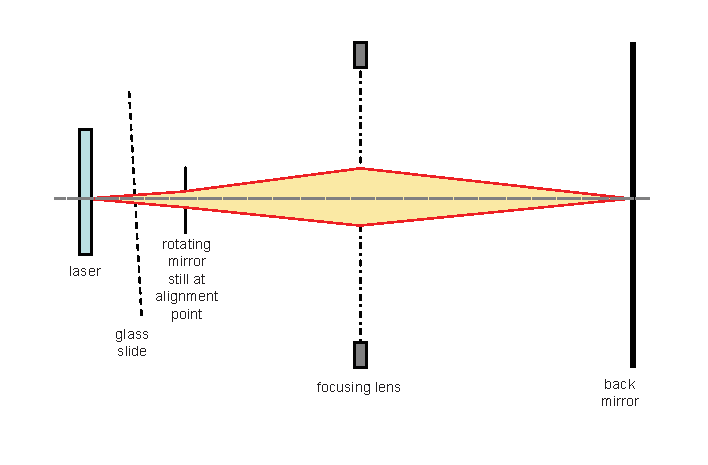
\includegraphics[width=3.8in]{clightoptics1.eps}
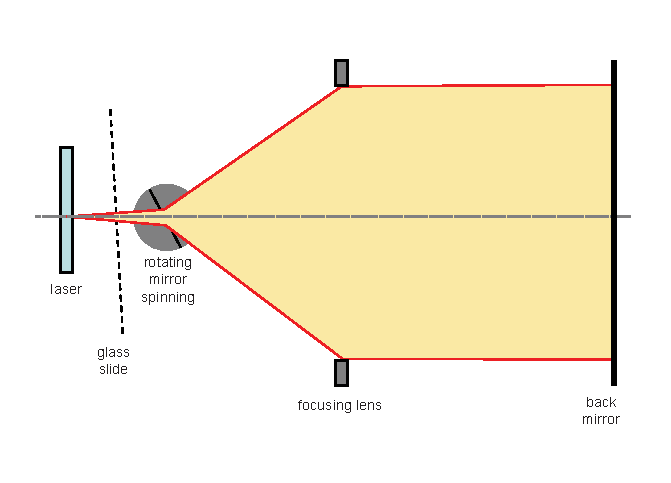
\includegraphics[width=3.8in]{clightoptics2.eps}
\caption{\label{clightoptics}
Unfolded diagrams of the optics of the experimental setup.  The vertical
scale has been expanded by a couple of orders of magnitude and the mirror
bends unfolded to straighten out the optical axis (gray horizontal line
across the middle of the above diagrams) to make the optics of the light
beam easier to visualize. 
The upper panel shows the beam when the rotating mirror is stationary in the
aligned orientation.  The focus of the laser spot has been placed on the back
mirror, so that the return beam envelope coincides with the outgoing beam 
envelope.  The lower panel shows what happens when the rotating mirror 
is spinning, fanning the beam out in the horizontal plane and filling the
aperture of the focusing lens.  Placing the lens so that the rotating mirror
is at its focus creates the parallel band between the lens and the back
mirror as shown, which gets focused back onto the frosted glass screen, as
shown.}
\end{figure}

One of the challenges in conducting this experiment is to optimize the
optics so that a small bright spot is visible on the frosted glass screen.
The beam from the laser is very bright, but it only passes
through the acceptance of the optics for a brief instant each time the
rotating mirror goes through 360$^{\circ}$.  At rotation frequencies above
30~Hz the spot looks continuous to the human observer, but decreased in
intensity by the fraction of the angular range of the mirror that is within
the acceptance of the optics, approximately 1/500 for the setup used in
this experiment.  Besides this, there is also some intensity lost at each
of the 5 mirror reflections, and another factor of approximately 10 at
the last reflection from the beam splitter.  What starts off as a 1~mW
beam from the laser is reduced to 100~nW average power by the time it
reaches the frosted screen, which can only be seen clearly by the human
eye in a low-background environment.  You will probably need to have the
lights in the laboratory turned off to get a clear view of the spot image
on the screen.

The path traveled by the beam through the optics is illustrated by the
optics diagrams in Fig.~\ref{clightoptics}.  The top panel in the figure
shows the conditions under which the light path is first aligned.  The
bends in the beam have been unfolded in the picture so that the central
ray of the beam, called the optical axis, is a straight line from the
laser to far mirror in the setup, which is labeled ``back mirror'' in the
diagram.  When the focusing lens is in the correct position, the source
object in the center of the laser is focused on the surface of the back
mirror.  This is achieved when the distances obey the following relation
to the focal length $f$ of the lens.
\begin{equation}
\frac{1}{f}=\frac{1}{a+r+s+b}+\frac{1}{d}
\label{eq:focus1}
\end{equation}
Under these conditions when everything is lined up, the reflected
beam envelope follows exactly the same profile as the outgoing beam, and
produces an image of the original laser spot back on the output window
of the laser.  If the distance from the beam splitter to the frosted glass
screen $s$ is set up to match the distance from the laser center to
the beam splitter, that same focused spot is imaged on the screen.  At this
point the spot is quite bright on the screen because the rotating mirror is
sitting still in the aligned position.

The lower panel in Fig.~\ref{clightoptics} indicates what happens to the
path of the light beam as soon as the rotating mirror starts spinning.
The view in the diagram is that of an observer looking down from the ceiling.
Note that the instantaneous beam spot is still a focused dot on the back
mirror, but it paints a stripe all the way across the back mirror when the
rotating mirror is spinning.  Optimum conditions for observation are achieved
when the rotating mirror is placed at the focus of the lens, so that the
fanned-out beam envelope becomes a parallel band between the lens and the
back mirror.  These conditions require that
\begin{equation}
f = a+b
\label{eq:focus2}
\end{equation}
There are enough variables in the set $r$,$s$,$a$,$b$,$d$ that
Eqs.~\ref{eq:focus1} and \ref{eq:focus2} can both be satisfied simultaneously
when your setup is properly aligned.

The round trip time for a light pulse to go from the rotating mirror to the
back mirror and return again to the rotating mirror is
\begin{equation}
t = 2\left(\frac{a+b+d}{v}\right)
\label{eq:t}
\end{equation}
where $v$ is the velocity of light in air. During this time, the rotating
mirror has moved through a small angle
\begin{equation}
\theta = \omega t
\label{eq:theta}
\end{equation}
where $\omega$ is the angular velocity of the rotating mirror. This results
in a displacement of the reflected spot on the front window of the laser by
the distance $y$
\begin{equation}
y=2(r+s)\theta
\label{eq:y}
\end{equation}
which translates to a displacement of the spot in the plane of the frosted
glass screen by distance $x$
\begin{equation}
x=\frac{2\theta(r+s)}{\sin{\alpha}}
\label{eq:x}
\end{equation}
where the angle $\alpha$ is indicated in Fig.~\ref{clightsetup}.
The data collection phase of the experiment consists of stepping through a
series of set rotation speeds of the mirror, and recording the position $x$
of the spot on the screen as a function of $\omega$.  Eqs.\ref{eq:t}-\ref{eq:x}
predict a linear relationship between $\omega$ and $x$.
\begin{equation}
x=\left(\frac{4(r+s)(a+b+d)}{v\sin{\alpha}}\right)\omega
\end{equation}
By fitting these data to a straight line and measuring the values for
$a$, $b$, $d$, $r$, and $s$, a measurement of the speed of light in air $v$
is achieved.

\section{Experimental Procedure}

All of the basic components of the setup shown in Fig.~\ref{clightsetup}
should be present at the beginning of the procedure, with the focusing lens
displaced out of the path of the beam.  Please the optical bench with the
laser mounted on it on a table at one end of the room, against the long wall
of the laboratory and pointing along the wall.  Mount the beam splitter on
the optical bench in the path of the laser beam so that it reflects the
outgoing beam against the back wall.  Mount the rotating mirror and motor
controller on a separate table located along the path of the laser.  Slide
the rotating mirror away from the laser until the laser beam spot is the
same diameter as the rotating mirror.  You can rotate the rotate the mirror
by hand by turning the large aluminum wheel attached to the drive motor. 
Be careful not to press on the thin mylar tape which serves as a drive belt
between the motor and the mirror spindle because it is fragile. 
Manually rotate the mirror so that the reflected beam is directed back toward
the laser and make sure that the height of the reflected beam passes a few cm
below the exit aperture of the laser.  These few cm of vertical misalignment
will make it easy later on to distinguish this directly reflected beam spot
from the one that passes through the entire optical path of the setup.

Determine the focal length $f$ of the focusing lens.  If the value is not
printed on the lens aperture, measure it by using the lens to focus the
rays of the sun down or some other distant light source.  The diameter of
the focused spot is a minimum when the image is formed a distance $f$ from
the lens.  If you do use the sun as a light source, chose a non-flammable
surface to image the spot so you do not ignite a fire.  Now place the first
fixed mirror back at the end of the room next to the laser table.  Be sure
to leave enough space between the laser table and the light path so that
the observers can work at the laser table without interrupting the beam or
bumping the mirror.  Then place the second fixed mirror near the far end of
the room, past where the rotating mirror table is located.
With the motor turned off,
carefully turn the rotating mirror until the beam is directed toward the
first fixed mirror.  Adjust the height of the mirror so that the beam spot
is centered.  Leave the rotating mirror untouched for the following alignment
steps.  Adjust the angle of the first fixed mirror to steer the reflected
beam onto the center of the second fixed mirror.  The second fixed mirror,
also called the back mirror, does not need to be at the same height as the
first mirror; in fact you may find that your setup is more stable if you
slide the back mirror down near the base of the stand, near the floor, and
align it there.

Next place the lens in the path of the beam a distance $f$ past the rotating
mirror along the outgoing beam path.  If $f$ is greater than $a$ then you
will place the lens past the first fixed mirror as shown in
Fig.~\ref{clightsetup}.  If it turns out in your setup that the lens belongs
before the first fixed mirror, the value of $b$ in Eqs.~\ref{eq:focus1}-
\ref{eq:focus2} will come out negative.  Once the lens is centered and
aligned with the beam axis, the beam will follow the same path it did 
before the lens was inserted, but the spot on the second fixed mirror will
appear much smaller.  Using a sheet of white paper, follow the focused
beam in the region in front of and behind the back mirror (you will need
to move the back mirror temporarily out of the beam) and try to find where
the focus is.  You may need the room lights turned out to carry out this
step.  If the focus seems to be past the wall, try moving the first fixed
mirror back until you can locate the focus inside the room.  You are done
with this step when the lens is located a distance $f$ downstream from the
rotating mirror along the light path, and the laser beam focus is on the
surface of the back mirror.  This is the condition described in 
Eqs.~\ref{eq:focus1} and \ref{eq:focus2}.

Once the back mirror has been correctly placed and the focused beam spot
centered on the back mirror, do not touch the first fixed mirror again.
The back mirror is equipped with special screws that allow fine adjustment
in its angles.  Have someone stand at the first fixed mirror and watch
as you adjust the angles on the back mirror to make the reflected beam
retrace its path back onto the first fixed mirror.  Two spots are visible
on the first fixed mirror, one made by the outgoing beam that remains in
one place, and the other made by the return beam that moves around when you
adjust the angles of the back mirror.  Use the fine adjustment screws on
the back mirror to exactly superimpose the reflected beam spot on top of the
original spot on the first fixed mirror.  When the two spots are exactly
on top of each other, the return beam will retrace the exact path followed
by the outgoing beam, all the way back to the laser.  Check that this is
true by looking for a red glow around the exit aperture of the laser.
Place the frosted glass screen on the laser table at the height of the
beam, and rotate the beam splitter until the reflected beam spot is centered
on the screen.

Measure the distances $r$, $s$, $a$, $b$, and $d$ shown in
Fig.~\ref{clightsetup}.  Check that Eqs.~\ref{eq:focus1} and \ref{eq:focus2}
are satisfied within errors.  If they are not, repeat the entire alignment
procedure from the beginning until both conditions are satisfied.  If the
agreement seems satisfactory but the agreement is outside the expected
range of 1-2 standard deviations, you may want to refine your estimates for
the distance measurement errors.  If two people are measuring a distance
with a tape measure, have the person holding the end of the tape first
center it on the measured surface to allow the other person to take a
reading, then pull it forward and back within an estimated margin of error
and have the other person record the difference as the measurement error.

Align the viewing telescope on the laser table so that it points in a
direction normal to the surface of the frosted screen.  You may rotate
the frosted screen to achieve this, but keep the angle $\alpha$ depicted
in Fig.~\ref{clightsetup} within 20$^{\circ}$ of 90$^{\circ}$ for optimum
visibility of the spot.  Once the splitter and the screen are set up,
record the value of $\alpha$ and do not touch either for the rest of the
experiment.  Now while an observer keeps an eye on beam spot on the frosted
screen, turn on the rotating mirror motor and set it to spin at a low speed.
As soon as the mirror starts to spin, the spot on the mirror will become
much dimmer, but it should appear in nearly the same place with the
same size and shape.  Now change the rotation speed of the mirror and
watch the spot move across the screen.  If you reverse the direction of
rotation of the mirror, the direction of displacement of the spot should
reverse.  If the spot does not appear to move, it is possible that you
are not looking at the right spot.  As a quick check have someone block
the beam by passing their hand in front of the back mirror and see if it
disappears.

Turn the translation stage of the viewing telescope to the middle of its
operating range.  Center the view of the telescope on the spot and adjust
the focus on the surface of the screen.  Once this is done, be careful not
to bump the position of the telescope for the remainder of the measurement.
Record the rotation speed of the mirror together with the reading of the
telescope translation stage.  Next increase the rotation speed of the mirror
by a small amount and notice that the spot has moved from the center of the
telescope viewport.  Advance the translation stage of the telescope until
the beam spot is centered again, using the central crosshair as a reference.
Record the new rotation speed and the new telescope translation stage reading.
Select a set of 8-10 different rotation motor speeds that cover the full
range of the motor controller, and step through them, recording the spot
position at each.  Then reverse the direction of the motor and repeat all
of the measurements.  At the end you should go back and step through a
subset of your measurements a second and third time.  This provides a
check that your results are reproducible, and also gives you a means to
estimate your measurement errors $\Delta x$.

One thing to keep in mind as you move the translation stage is that in
order to get reliable readings, you always need to advance to the centered
position from the same direction.  This is because there is considerable
play in the worm gear that moves the carriage, and every time you switch
direction, the spindle rotates through a number of turns before it
engages and begins to move the carriage.  The effect is called {\em backlash}.
To avoid large position uncertainties caused by backlash, make sure that
you always make your approach into the alignment position from the
same direction, either advancing to the right or to the left.  If your
first set of measurements were taken with increasing speed in the clockwise
direction, then when you switch to counter-clockwise rotation you may want
to start at the high-frequency end of the range and work down so that you
always advance the translation stage in the same direction.  To prevent
damage to the motor and mirror drive belt, avoid running the mirror above
1000~Hz continuously for more than about a minute.

Fit the data $x\pm \Delta x$ vs $\omega$ to a straight line and
extract the best-fit slope parameter together with its error.  Remember
that the angular frequency $\omega$ is related to the rotating frequency
measured in Hz through a factor of $2\pi$.  Check
that the $\chi^2$ value from the fit is consistent with expectations
based on the number of degrees of freedom in the fit, verifying whether
or not your data are consistent with a linear relationship between $\omega$
and $x$.
Use Eq.~\ref{eq:x} to convert the slope to a value for $v$, together with
its error.  Do not forget to include the errors on the distance measurements
in computing the error on $v$.  Compare your result with the published
value for the speed of light in vacuum $c=2.99792458$~m/s.

%\begin{table}
%\caption{\label{displacementfig}
%Nkmg cktetchv cpf dtkfigu, cpf vq uocnngt uvtwevwtgu
%nkmgcvqou cpf pwengk, vjku ukorng oqfgn ikxgu korqtvcpv kpukijv kpvq
%vjgdgjcxkqt qh gxgp vjg oquv eqornkecvgf uauvgou yjgp vjgkt fapcokeu
%ctgiqxgtpgf da uocnn fgrctvwtgu htqo gswknkdtkwo.}
%\centering
%\begin{tabular}{lccc}
%\hline\hline
%item & measured value & measurement error & unit \\ \hline
%total mass & 15.67 & 0.02 & kg \\
%length eyes-tailfin & 14.6 & 0.05 & cm \\
%height belly-dorsal & 3.98 & 0.05 & cm \\
%flash response time & 1.23 & 0.15 & s \\
%total turn time & 1.08 & 0.05 & s \\
%turn radius & 0.72 & 0.15 & cm \\
%maximum turn velocity & 22.1 & 0.5 & m/s \\
%\hline\hline
%\end{tabular}
%\end{table}

%\begin{figure}
%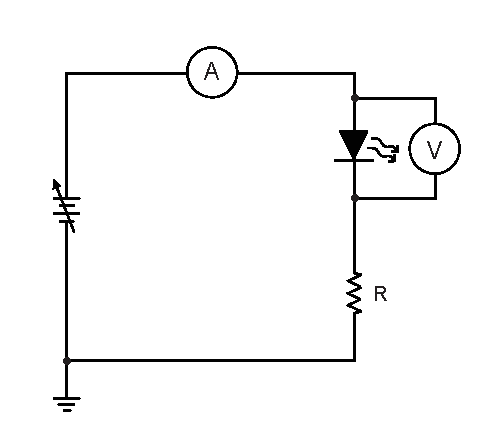
\includegraphics[width=2in]{VIcircuit.eps}
%\caption{\label{VIcircuit}
%Diagram of the circuit used to measure V-I curves for the LEDs examined
%in this experiment.  The resistor $R$ is present to protect the LED against
%accidental over-voltage.  Its value should be no less than 100~$\Omega$.}
%\end{figure}

\begin{acknowledgments}
This document was updated by Prof. Richard Jones, based on an original
write-up by Prof. Doug Hamilton (1987).
\end{acknowledgments}

%% Create the reference section using BibTeX:
%\bibliography{revtex4}

\begin{thebibliography}{9}

\bibitem{Bates88}
H.E. Bates, {\em Recent measurements of the speed of light and the
redefinition of the meter}, Am.  J. Phys. {\bf 56} (1988) p. 682.
\end{thebibliography}

\end{document}
%%
%% ****** End of file template.aps ******
%
%
